% ================================================================================================================================================== %

\documentclass[runningheads,a4paper]{llncs}

\usepackage{verbatim}
\usepackage{amssymb}
\setcounter{tocdepth}{3}
\usepackage{graphicx} % Used for inserting pdf as graphics
\usepackage{float} % Used fo0r 'H' float option in figures
\usepackage{hyperref} % Used for creating a hyperlink to reference parts
\usepackage{enumitem}
\usepackage{textcomp}
\usepackage{multicol}

\usepackage{multirow}
\usepackage{url}
\usepackage{color}
\urldef{\mailsa}\path|radelacruz@up.edu.ph|
\urldef{\mailsb}\path|fccabarle@up.edu.ph|
\urldef{\mailsc}\path|ivan.cedric10@gmail.com|
\urldef{\mailsd}\path|hnadorna@dcs.upd.edu.ph|
\urldef{\mailse}\path|zxxhust@gmail.com|
\usepackage{mathtools}
\DeclarePairedDelimiter\ceil{\lceil}{\rceil}
\DeclarePairedDelimiter\floor{\lfloor}{\rfloor}
    
\newcommand{\keywords}[1]{\par\addvspace\baselineskip
\noindent\keywordname\enspace\ignorespaces#1}
%\newcommand{\tt}[1]{\texttt{#1}}

\begin{document}


\mainmatter


\title
{
Homogeneous Spiking Neural P Systems with Structural Plasticity
}

\titlerunning
{
Homogeneous SNPSP Systems
}


\author
{
Ren Tristan A. de la Cruz$^1$
\and
Francis George C. Cabarle$^{1,2}$
\and
Iva Cedric H. Macababayao$^{1}$
\and
Henry N. Adorna$^1$ 
\and
Xiangxiang Zeng$^3$
}

\authorrunning {de la Cruz et al}


\institute
{
$^1$Algorithms and Complexity Laboratory \\
Department of Computer Science, University of the Philippines - Diliman\\
Diliman 1101, Quezon City, Philippines    \\
$^2$Shenzhen Research Institute of Xiamen University \\
Xiamen University, Shenzhen 518000, Guangdong, China.\\
$^3$ School of Information Science and Engineering\\
Hunan University 410082, Changsha, China \\
%\mailsa , \mailsb, \mailsc, \mailsd, \mailse 
}


\toctitle{Lecture Notes in Computer Science}
\tocauthor{Authors' Instructions}


\maketitle


% ================================================================================================================================================== %



\begin{abstract}

Spiking neural P system (SNP System) is a model of computation inspired by the mechanism of a spiking neuron. An SNP system is a network of neurons
that can communicate with each other using an object known as a spike (the object spike represents action potential or nerve impulse).  Spiking neural 
P systems with structural plasticity (SNPSP system) is a variant of the SNP system model. It incorporates the concept of structural plasticity to the
SNP system model. SNPSP systems have the ability to add and delete connections between neurons. In SNPSP systems, the behavior of a neuron can be
``programmed" by giving it a set of rules. Different set of rules will result in different behaviors. In this work, we show that it is possible to
construct a universal SNPSP system where all the neurons in the system use the same set of rules. Such systems are called homogeneous SNPSP systems.

\keywords{Membrane Computing, 
          Spiking Neural P Systems, 
          Homogeneous Neurons,
          Structural Plasticity}
\end{abstract}



% ================================================================================================================================================== %



\section{Introduction}

\textit{Membrane computing} is an area of theorical computer science that studies family of related models of computation known as \textit{P systems}.
\textit{P systems} are unconventional models of computation that are biologically-inspired (see \cite{HANDBOOK}. They were introduced formally by 
Gheorghe P\u{a}un in \cite{mc} (the `P' in P systems stands for P\u{a}un). P systems are inspired by biological cells' mechanisms. They include models
that are inspired by the internal works of a cell (cell-like systems), models inspired by a group of cells (tissue-like systems), and models inspired 
by group of neurons (neural-like systems).


Neural-like P systems known as \textit{spiking neural P systems} (SNP systems) were introduced in \cite{SNP}. They are inspired by the workings of a
network of spiking neuron. The computing elements (processors) of SNP systems are called \textit{neurons}. The neurons also store information, each
neuron can store a multiset of object called a \textit{spike}. An SNP system is a network of such neurons. The neurons are connected to each other 
using \textit{synapses}. We sometime will refer to this model as \textit{classic} or \textit{standard} SNP system since there are already a lot of
SNP system variants that have been introduced.

The standard SNP system is based on an simplified and highly abstracted mechanisms of a spiking neuron. There are many features in the brain that are 
good sources of inspiration for the creating of new variants of SNP systems. \textit{e.g.} inhibitory impulses, weighted synapses, neuron division, 
threshold mechanism, astrocytes, neuron budding, axons, \emph{etc}. Many variants of SNP systems that use these features have been introduced (see 
\cite{pan-snpweight-2012,paun-astroc-snp-2007,song-snp-syn-2014,wang-snpweights-2010,pan-anti-snp-2009,pan-astro-snp-2012,wu-cellsnp-2016,SNPwT,song-pan-rulsyn-maxspik-2015,AXONP}).

In this work, we going to focus on a variant of SNP system is known as \textit{spiking neural P system with structural plasticity} (SNPSP system) 
introduced in \cite{SNPSP}. SNPSP system uses the feature of the brain known as  \textit{structural plasticity}. Structural plasticity is the ability
of the brain to rewire itself. Structural plasticity includes \textit{synaptogenesis} and \textit{synaptic pruning}. Synaptogenesis is the creation of 
synapses while synaptic pruning is the deletion of existing synapses. These features give the SNPSP systems the ability to change their structure 
which is not possible for standard SNP systems and some other variants.

A neurons in an SNPSP system can be ``programmed" by giving them a set of rules. Different neurons can be programmed differently by giving them 
different sets of rules. The purpose of this work is to show that a universal SNPSP system can be constructed in such a way that all the neurons in
the system use the same set of rules. We call such systems as \textit{homogeneous} SNPSP systems. It has been shown that universal homogeneous systems
can be constructed using different SNP variants (see \cite{HSNP}, \cite{HISNP}, \cite{HSNP-R}, \cite{HSNP-S}, \cite{HSNP-A}).

This work is organized as follows: In Section \ref{sec-prelims} we introduced premilinary concepts need to understand the main results namely the
basics of formal languages and regular language in Section \ref{sec-lang-reg} and the concept or register machines in Section \ref{sec-register}. In
Section \ref{sec-snpsp} we formally define an SNPSP system. Section \ref{homogeneous-snpsp} contains the two main results of this work, the 
construction of universal homogeneous SNPSP systems. Section \ref{sec-disc} contains the discussion of the results and some conclusions.

% ================================================================================================================================================== %



\section{Preliminaries} \label{sec-prelims}


\subsection{Languages and Regular Languages} \label{sec-lang-reg}

An alphabet $V$ is a finite set of symbols, a string $s$ is a concatenation of symbols from some $V$, so that the string is said to be \textit{over
the alphabet} $V$. If $s$ is a string over $V$, we denote as $|s|$ the length of $s$ while $|s|_a$ where $a \in V$ denotes the number of occurrences 
of symbol $a$ in $s$. 
  
A language $L$ is a set of strings. When talking about languages, the term \textit{word} can be
used as a synonym for string. For some alphabet $V$ we have $V^*$ as the language that contains
strings of all lengths over $V$ including the empty string, denoted as $\lambda$. Further, 
$V^+ = V^* - \{\lambda\}$. 

In defining a specific type of language known as \textit{regular languages}, we can use
\textit{regular expressions}. We define regular expressions in an iterative manner over an alphabet
$V$, as follows: (1) each $a \in V$ and $\emptyset$ are regular expressions, (2) if $E_1$ and $E_2$ are regular expressions, then $E_1 \cup E_2$,
$E_1 E_2$, and $E_1^*$ are also regular expressions. The language defined by a regular expression $E$ is denoted as $L(E)$. If $E_1$ is a regular
expression $E_1 = a$ where  $a \in V$, then the language $L(E_1)$ is $\{a\}$. The language defined by regular expression $\emptyset$ is the empty
language $\{\}$. Given regular expressions $E_1$ and $E_2$ and the languages they define, $L(E_1)$ and $L(E_2)$ respectively, the language
defined by regular expression $E_1 \cup E_2$ is  $L(E_1 \cup E_2) =L(E_1) \cup L(E_2)$, the language defined by regular expression $E_1 E_2$
is $L(E_1 E_2) = \{xy|x \in L(E_1) \text{ and } y \in L(E_2) \}$, and the language defined by regular expression $E_1^*$ is $L(E_1^*) = \{xy|
x \in L(E_1) \cup \{\lambda\} \text{ and } y \in L(E_1^*)\}$. 

% ================================================================================================================================================== %

\subsection{Register Machines}\label{sec-register}

\textit{Register machines}, also known in literature as counter machines or program machines, are models of computation that use \textit{registers} to
store information (non-negative integers). The particular register machine model that we will use is the same register machine model described in 
Section 3 in \cite{SNP}. This register machine performs two main types of instruction: $ADD$ and $SUB$. An $ADD$ instruction increases the value 
stored in a specified register by 1 while a $SUB$ instruction decreases the value in a specified register by 1 (if the value is not yet 0). A third 
type of  instruction known as $HALT$ will stop the entire operation of the machine when executed.
    
Formally, a register machine $M$ is a construct $M = (m, H, l_0, l_h, I)$, where:
  
\begin{itemize}  
   \item $m$ is the number of registers.    
   \item $H$ is the set of instruction labels.    
   \item $l_0$ is the label of the initial instruction.
   \item $l_h$ is the label of the $HALT$ instruction.
   \item $I$ is the set of all instructions.    
\end{itemize}

An instruction label from $H$ labels only one instruction from $I$. The instructions have the following forms and semantic meaning:

\begin{itemize}
   \item $l_i: (ADD(r),l_j,l_k)$. Increase the value stored in register $r$ by 1 then non-deterministically select the label of the next instruction
         from $\{l_j,l_k\}$.         
   \item $l_i: (SUB(r),l_j,l_k)$. Decrease the value stored in register $r$ by 1 if the value is not zero. The next instruction will then be the 
         instruction labeled as $l_j$. If the value in register $r$ is zero, then simply proceed to the next instruction labeled $l_k$.
   \item $l_h: HALT$. Stop the operation of the machine.
\end{itemize}
  
In \textit{generating mode}, the computation of a register machine $M$ is as follows: $M$ starts with all its registers empty (all the registers store
zero) and executes the instruction labeled as $l_0$. The machine will continue to execute instructions until it executes the halt instruction labeled
as $l_h$. If the machine halts, then the value in the first register is said to be \textit{generated} by the machine $M$. $N(M)$ denotes the set of 
numbers generated by machine $M$. 
  
In \textit{accepting mode}, register machines can \textit{accept} numbers instead of generating them. The machine works as follows: a number is 
introduced in a specified register, and then the machine will begin by executing instruction labeled $l_0$. If eventually the machine halts by 
executing instruction labeled $l_h$, then the number that was introduced in the specified register is said to be accepted. If there is no confusion, 
we also denote as $N(M)$ the set of numbers accepted by machine $M$.

It has been proven in \cite{MINSKY} that register machines compute (generate/accept) sets of numbers that are computable using Turing machines
(denoted as $NRE$). 
  
% ================================================================================================================================================== %

\section{Spiking Neural P Systems with Structural Plasticity}\label{sec-snpsp}

Spiking neural P system with structural plasticity (SNPSP system) is a variant of the classic spiking neural P system (SNP system) model. SNPSP 
systems were introduced in \cite{SNPSP}. Formally, an SNPSP system $\Pi$ of degree $m \geq 1$ is  {a} construct: $\Pi =(O, \sigma_1,\ldots, \sigma_m, 
syn, in, out)$, where:

\begin{itemize}[label=$\circ$]
   \item  $O = \{a\}$ is a singleton alphabet containing only the symbol $a$. $a$ is called a \textit{spike}.
   \item $\sigma_1, \ldots, \sigma_m$ are the \textit{neurons} of the system. A neuron $i$ ($1 \leq i \leq m$) has the form $\sigma_i = (n_i, R_i)$. 
          $n_i$ is a non-negative integer that indicates the initial number of spikes in $\sigma_i$. $n_i$ is represented by the string $a^{n_i}$. 
          $R_i$ is a finite set of rules with the following forms:
          \begin{itemize}
             \item \textbf{Spiking Rule:} $E/a^c \rightarrow a$ where $E$ is a regular expression over $O$ and $c \geq 1$. When $E=a^c$, the rule can 
                   be written as $a^c \rightarrow a$.
             \item \textbf{Plasticity Rule:} $E/a^c \rightarrow \alpha k(i,N)$ where $c \geq 1$, $\alpha \in \{+,-,\pm,\mp\}$, $N \subseteq \{1,
                   \ldots,m\}-\{i\}$, and  $1 \leq k \leq |N|$. When $E=a^c$, the rule can be written as $a^c \rightarrow \alpha k(i,N)$.
          \end{itemize}
   \item $syn \subseteq \{1,\ldots,m\} \times \{1,\ldots,m\}$, with $(i,i) \not\in syn$, is the set of initial \textit{synapses} between neurons.
   \item $in,out$ are neuron labels that indicate the input and output neurons respectively.
\end{itemize}
  
% ================================================================================================================================================== %

 
For each time step, each neuron of will check if any of its rules are applicable. $E/a^c$ (part of the rule) specifies the two conditions for a rule
to be applicable. A rule is applicable only if (1) the string $a^{n_i}$ is in $L(E)$ and  (2) $n_i \geq c$ where $n_i$ is the number of spike in the
neuron.

It is possible that multiple rules are applicable in a neuron. This occurs when the languages defined by the regular expressions of the rules 
intersect. i.e. \texttt{rule 1}: $E_1/a^{c_1} \rightarrow a$, \texttt{rule 2}: $E_2/a^{c_2} \rightarrow a$ and $L(E_1) \cap L(E_2) \neq \varnothing$. 
If multiple rules are applicable in a neuron, the neuron will non-deterministically select one rule to activate. If a rule is activated in $\sigma_i$,
$c$ spikes are consumed leaving $\sigma_i$ with $n_i-c$ spikes.
  
If a spiking rule is activated at $\sigma_i$, all $\sigma_j$'s such that $(i,j) \in syn$ will receive a spike from $\sigma_i$.
  
If a plasticity rule $E/a^c \rightarrow \alpha k(i, {N})$ is activated in $\sigma_i$, the neuron will perform one of the following actions:
\begin{itemize}
   \item If $\alpha = +$. Add a set of $k$ synapses connecting $\sigma_i$ to some $k$ neurons whose labels are specified in $N$. (``+ action")
   \item If $\alpha = -$. Delete a set of $k$ synapses that connect $\sigma_i$ to some $k$ neurons whose labels are specified in $N$. (``- action")
   \item If $\alpha = \pm$. At rule activation time $t$, perform the \textit{``+ action"}, then at time $t+1$ perform the \textit{``- action"}.
   \item If $\alpha = \mp$. At rule activation time $t$, perform the \textit{``- action"}, then at time $t+1$ perform the \textit{``+ action"}.
\end{itemize}
  
Let $P(i) = \{j|(i,j)\in syn\}$. Let us call $P(i)$ the set of labels of ``already connected neurons" ($\sigma_j$'s are ``already connected" to 
$\sigma_i$ via synapses $(i,j)$'s). Let us call $N$ (specified in any plasticity rule) the set of labels of ``target neurons".

When performing the \textit{``+ action"} ($\alpha = +$), the set of labels that is relevant is the set $N-P(i)$. We only want the neuron labels 
in $N$ that do not specify neurons that are ``already connected" to $\sigma_i$. We call $N-P(i)$  the set of labels for ``feasible target neurons". 
i.e. $x$ is a label of a ``feasible target neuron" if $x \in N$ and $x \not\in P(i)$. There are 3 possible scenarios when it comes to the size of
set of labels for ``feasible target neurons". 
\begin{enumerate}
   \item $|N-P(i)| < k$. The number of feasible target neurons is less than number of synapses ($k$) that the rule wants to create. In this scenario,
         the rule will only create less than $k$ synapses connecting $\sigma_i$ to $|N-P(i)|$ feasible target neurons from $N-P(i)$.
   \item $|N-P(i)| = k$. The number of feasible target neurons is exactly the number of synapses ($k$) that the rule wants to create. In this 
         scenario, the rule will create exactly $k$ synapses connecting $\sigma_i$ to $k$ feasible target neurons from $N-P(i)$.
   \item $|N-P(i)| > k$. The number of feasible target neurons is greater than the number of synapses ($k$) that the rule wants to create. In this 
         scenario, the rule will create exactly $k$ synapses connecting $\sigma_i$ to $k$ non-deterministically selected feasible target neurons from 
         $N-P(i)$.
\end{enumerate}

When performing the \textit{``- action"} ($\alpha = -$), the set of labels that is relevant is the set $N \cap P(i)$. We only want the neuron labels 
in $N$ that specify neurons that are ``already connected" to $\sigma_i$. We call $N \cap P(i)$  the set of labels for ``feasible target neurons". 
i.e. $x$ is a label of a ``feasible target neuron" if $x \in N$ and $x \in P(i)$. There are 3 possible scenarios when it comes to the size of
set of labels for ``feasible target neurons". 
\begin{enumerate}
   \item $|N \cap P(i)| < k$. The number of feasible target neurons is less than number of synapses ($k$) that the rule wants to delete. In this
         scenario, the rule will only delete less than $k$ synapses that connect $\sigma_i$ to $|N \cap P(i)|$ feasible target neurons from $N \cap 
         P(i)$.
   \item $|N \cap P(i)| = k$. The number of feasible target neurons is exactly the number of synapses ($k$) that the rule wants to delete. In this 
         scenario, the rule will delete exactly $k$ synapses that connect $\sigma_i$ to $k$ feasible target neurons from $N \cap P(i)$.
   \item $|N \cap P(i)| > k$. The number of feasible target neurons is greater than the number of synapses ($k$) that the rule wants to delete. In 
         this scenario, the rule will delete exactly $k$ synapses that connect $\sigma_i$ to $k$ non-deterministically selected feasible target 
         from $N \cap P(i)$.
\end{enumerate}

We note that creation of a synapse from $\sigma_i$ to $\sigma_j$ will also result in $\sigma_j$ receiving a spike. 
  
A plasticity rule with $\alpha \in \{\pm,\mp\}$ will be active for two time steps. When such rule is activated at time $t$, it will be active until 
time $t+1$. During time $t$ and $t+1$ no other rules can be activated but the neuron can still receive spikes. It is only at time $t+2$ when another
rule can be activated. 

A configuration of an SNPSP system at time $t$ is defined by (a) number of spikes in each neuron at time $t$ and (b) set of synapses at time $t$. 
We can represent (a) as the vector $C^t = \langle n_1^t, n_2^t, ...,n_m^t\rangle$ where $n_i^t$ is the number of spikes in $\sigma_i$ at time $t$.
We can represent (b) as the set $syn^t$ that contains all synapses in the system at time $t$.

In \textit{generating mode}, we observe the system's output neuron, $\sigma_{out}$. $\sigma_{out}$ is said to have a synapse to the $
\textit{environment}$. In SNP or SNPSP system, we can think of the environment as a neuron that is not part of the system but can receive spikes
from the system via the synapse connecting the output neuron to the environment. We consider the first two spikes sent by $\sigma_{out}$ to the environment.
If the first spike is sent at time $t_1$ and the second spike is sent at time $t_2$, then the output (generated number) of the system for that 
specific computation (run) is the time difference $n=t_2-t_1$. $N_2(\Pi)$ is the set of numbers generated by system  $\Pi$ for all halting
computation.

In \textit{accepting mode}, we use the input neuron, $\sigma_{in}$. $\sigma_{in}$ will accept two spikes from the environment. If the first spike is
received by $\sigma_{in}$ at time $t_1$ and the second spike is received at time $t_2$, then the input (number) to the system is the time difference 
$n=t_2-t_1$. The input is accepted by system $\Pi$ if eventually the system halts.  $N_{acc}(\Pi)$ is the set of numbers accepted by system $\Pi$.

$N_xSNPSP$ is the family of all sets $N_x(\Pi)$ where $x \in \{2, acc\}$ such that $\Pi$ is an SNPSP system.

There are other ways of interpreting the output of an SNPSP system. One can count the total number of spikes the output neuron sends to the
environment and say that the number is the output of the system. For every time step, we can also observe the synapse from the output neuron to the
environment, if the output neuron spikes the system is said to output `1' at that time step otherwise the system is said to output `0'. The string
(spike train) generated by output neuron can be interpreted as the output of the system.

% ================================================================================================================================================== %

\subsection{SNPSP System's `Forgetting Rule'} \label{sec-forget}

There is a rule type in SNP systems known as \textit{forgetting rule}. A \textit{forgetting rule} has the form $a^s \rightarrow \lambda$. The rule
can be applied when the neuron contains $s$ spikes. If activated, a forgetting rule simply consumes $s$ spikes on the same step the rule was activated
. The behavior of a forgetting rule can be simulated using SNPSP system's plasticity rule. A plasticity rule of the form $E/a^s \rightarrow 
-1(i,\{x\})$ will behave exactly like a forgetting rule if synapse $(i,x)$ does not exist and $E=a^s$. When activated, the plasticity rule consumes 
$s$ spikes and it attempts to delete one synapse (since $\alpha = -, k=1$) connecting $\sigma_i$ to $\sigma_x$. If the synapse $(i,x)$ does not exist, 
then the plasticity rule simply consumes the $s$ spikes needed for the rule to activate. For brevity we adopt the notation for forgetting rule by
writing plasticity rules that simply consume spikes as $E/a^s \rightarrow \lambda$. 

In SNP systems, a forgetting rule is restricted to the form $a^s/a^s \rightarrow \lambda$ (simply written as $a^s \rightarrow \lambda$). The regular
expression $E$ of the rule is always $a^s$ where $s$ is also the number of spikes consumed. We do not have this restriction for SNPSP systems. Our 
version of the `forgetting rule' is technically a plasticity rule so we can have any regular expression. Another SNP system restriction is that in a 
given neuron, the language defined by regular expression of any forgetting rule should not intersect with the language defined regular expression of 
any of the spiking rule. i.e. No spiking rule and forgetting rule can be applicable at the same time. We also do not have such restriction for SNPSP
systems. SNPSP system's `forgetting rule' is a plasticity rule whose regular expression can intersect while regular expression of some spiking rule.
i.e. It is possible for an SNPSP system's `forgetting rule' to be applicable at the same time as some spiking rule. This makes an SNPSP system's 
`forgetting' rule a generalized version of SNP system's forgetting rule.

We are going to use SNPSP system's `forgetting rules' to prove the main results of this work.

% ================================================================================================================================================== %

\section{Homogeneous Spiking Neural P Systems with Structural Plasticity} \label{homogeneous-snpsp}

% ================================================================================================================================================== %

\subsection{Homogeneity of an SNPSP System}

We call an SNPSP system $\Pi$ \textit{homogeneous} if all the neurons in the system have the same set of rules. That is, $R_1 = R_2 = ... = R_m$
for $\sigma_i = (n_i, R_i)$ in system $\Pi$. $N_xHSNPSP$ is the family of all sets $N_x(\Pi)$ with $x \in \{2, acc\}$ such that $\Pi$ is a homogeneous
SNPSP system.  

In the following sections, the only plasticity rules that we are going to use are the ones the simulate SNP system's forgetting rule (as described in
Section \ref{sec-forget}). Specifically, we are going to use plasticity rules of the form $E/a^c \rightarrow -1(i,\{w\})$ where $i$ is the label of
the neuron that contains the rule and $\sigma_w$ is an isolated neuron with no incoming or outgoing synapses. In Section \ref{sec-forget}, we write
such rules as $E/a^c \rightarrow \lambda$. 

Due to the syntax of plasticity rule ($E/a^c \rightarrow \alpha k (i, N)$), technically, no two plasticity rules from different neurons can be the
same. i.e. In a system $\Pi$, if there are two SNPSP system `forgetting' rules, one in $\sigma_y$ and another in $\sigma_z$, then the `forgetting'
rule in $\sigma_y$ is technically  $E/a^c \rightarrow -1(y,\{w\})$ while the `forgetting' rule in $\sigma_z$ is technically $E/a^c \rightarrow -1(z,
\{w\})$. Both rules have the same regular expression ($E$), consume the same amount ($c$) of spikes, and perform the same operation (defined 
$\alpha = -, k=1, N=\{w\}$). The only difference between the two rules is the $i$ which specifies the label of the neuron where the rule is located.
If $i$ (which specifies the neuron containing the rule) is the only difference between a plasticity rule from one neuron to another plasticity rule
in another neuron, then we consider those two rules as the same rule since their behavior is the same.

% ================================================================================================================================================== %

\subsection{Universality of Homogeneous SNPSP Systems in Generating Mode}\label{sec-gen-mode}

\begin{theorem}\label{theorem-1}
$NRE = N_2HSNPSP$ 
\end{theorem}

\proof To prove Theorem \ref{theorem-1}, we will show that $NRE \subseteq N_2HSNPSP$. For the converse inclusion $N_2HSNPSP \subseteq NRE$, we can
invoked the Church-Turing thesis and state that for any set $S$ (of numbers) in $N_2HSNPSP$, a Turing machine can be constructed the computes set $S$. 
In Section \ref{sec-register}, we mentioned that register machines  working in generating mode can characterize $NRE$. By showing that a homogeneous
SNPSP system $\Pi$ can simulate register machine $M=(m, H, l_0, l_h, I)$ we can show that $NRE \subseteq N_2HSNPSP$.

Given the register machine $M$, we will construct a homogeneous SNPSP system $\Pi$ that simulates the behavior of $M$. SNPSP system $\Pi'$ 
is constructed by creating different modules that will simulate parts of register machine $M$. The SNPSP modules are:
(1)  ADD module: Each ADD instruction $l_i$ will have a corresponding SNPSP ADD module.
(2)  SUB module: Each SUB instruction $l'_i$ will have a corresponding SNPSP SUB module. 
(3)  HALT module: Single HALT instruction $l_h$ will have the corresponding SNPSP HALT module.
(4)  OUT module: System $\Pi$ will have an SNPSP OUT module that will help transform the store output (number) to an output spike train.


Table \ref{table-rules} shows the rule set that will be used by all the neuron in the system. $x,y,z$ are constant values that will be specified
later.

\begin{table}[H]
\begin{center}
\begin{tabular}{|r|l|}
\hline
\tt{Rule 0}  & $a^{x+1}/a          \rightarrow \lambda$  \\ 
\tt{Rule 1}  & $a^{x+2}/a^2        \rightarrow \lambda$  \\ 
\tt{Rule 2}  & $a^{x+2}/a^2        \rightarrow a$        \\ \hline 
\tt{Rule 3}  & $a^{y+1}/a          \rightarrow \lambda$  \\ 
\tt{Rule 4}  & $a^{y+2}/a^2        \rightarrow a$        \\ \hline
\tt{Rule 5}  & $a^{z+1}/a          \rightarrow a$        \\ 
\tt{Rule 6}  & $a^{z+2}/a^2        \rightarrow \lambda$  \\ 
\tt{Rule 7}  & $a^{z+1}(a^3)^+/a^4 \rightarrow \lambda$  \\
\tt{Rule 8}  & $a^{z+2}(a^3)^+/a^3 \rightarrow a$        \\ \hline
\end{tabular}
\end{center}
\caption{Rule Set for All Neurons in System $\Pi$}
\label{table-rules}
\end{table}


% ================================================================================================================================================== %

An ADD module for instruction $l_i:(ADD(r), l_j, l_k)$ has the following 6 neurons: $l_{i,1}$, $l_{i,2}$, $l_{i,3}$, $l_{i,4}$, $l_{i,5}$, $l_{i,6}$.
The structure of the ADD module and the initial spikes in neurons are shown in Figure \ref{fig-add}. Neuron $r$ represents register \texttt{r}. If 
register $r$ stores number $n$, then neuron $r$ will store $z+3n$. e.g. Number 0 is represented as $z$ spikes in neuron $r$, number $5$ is represented 
as $z+3(5)=z+15$ spikes, and number $9$ is represented as $z+3(9)=z+27$ spikes. The  $x,y,z$ values for the initial spike counts are the same 
constants used in the rules. We will specify their values later.

\begin{figure}
\begin{center}
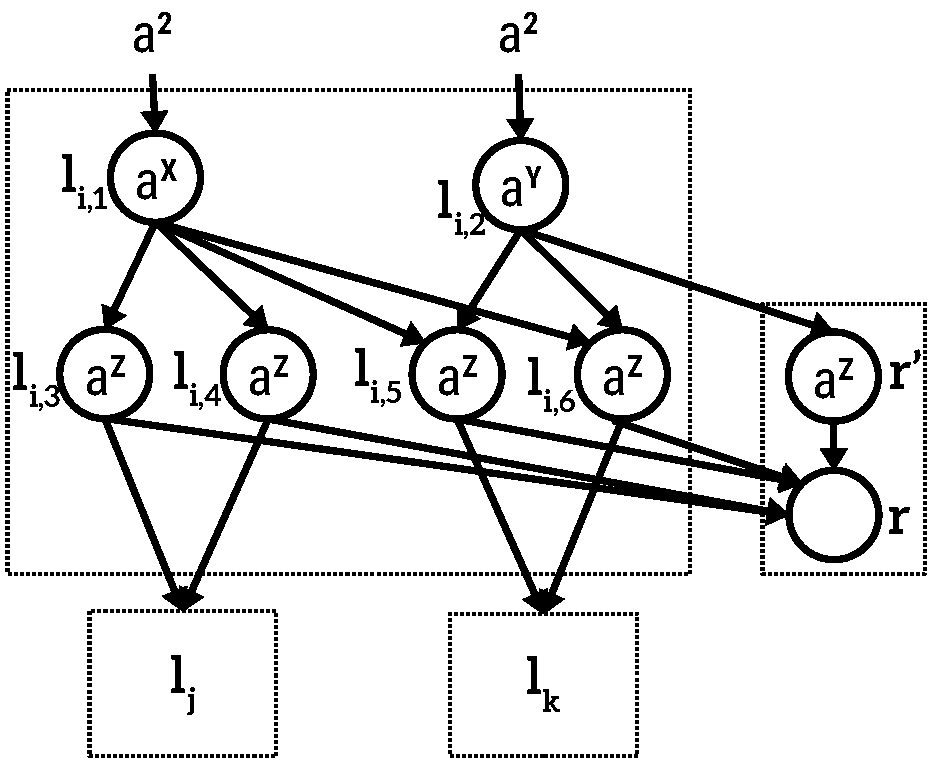
\includegraphics[scale=0.50]{figures/add-module-2.pdf}
\caption{ADD Module for Simulating Instruction $l_i:(ADD(r), l_j, l_k)$}
\label{fig-add}
\end{center}
\end{figure}   

The ADD operation is triggered by sending 2 spikes each to neurons $l_{i,1}$ and ${l_{i,2}}$. We call neurons $l_{i,1}, l_{i,2}$ the `starting neurons'
of the module. Let $t$ be the time the spikes are received. The ADD operation works as follows:
\begin{itemize}
   \item Time: $(t+1)$. From the initial spike count $x$, neuron $l_{i,1}$ has now $x+2$ spikes and will non-deterministically select either 
                        \texttt{Rule 1}: $a^{x+2}/a^2 \rightarrow \lambda$ or \texttt{Rule 2}: $a^{x+2}/a^2 \rightarrow a$. Either rule will consume
                        2 spikes returning the spike count of the neuron to $x$. If \texttt{Rule 2} is activated, then neuron $l_{i,1}$ will send a 
                        spike each to neurons $l_{i,3}$, $l_{i,4}$, $l_{i,5}$, $l_{i,6}$.
   \item Time: $(t+1)$. From initial $y$ spikes, neuron $l_{i,2}$ has now $y+2$ spikes and will use \texttt{Rule 4}: $a^{y+2}/a^2 \rightarrow a$ 
                        consuming two spikes and sending a spike each to neurons $l_{i,5}$, $l_{i,6}$, $r'$.

   \item Time: $(t+2)$. For this case, we consider the situation where neuron $l_{i,1}$ used \texttt{Rule 1}: $a^{x+2}/a^2 \rightarrow \lambda$. 
                        Neurons $l_{i,3}$ and $l_{i,4}$ will not receive any spikes. Neurons $l_{i,5}$, $l_{i,6}, r'$, from the initial $z$ spikes, 
                        will now have $z+1$ spikes each (the additional spike being from neuron $l_{i,2}$). Neurons $l_{i,5}$, $l_{i,6}, r'$ will all
                        use \texttt{Rule 5}: $a^{z+1}/a \rightarrow a$ returning their spike count to $z$ and each of them sending a spike to neuron 
                        $r$. This will increment the number of spikes in neuron $r$ by 3 spikes which means the number $n$ stored in register $r$ is 
                        incremented by 1. Neurons $l_{i,5}$ and $l_{i,6}$ will send $2$ spikes to starting neuron(s) of module $l_k$ triggering its 
                        operation.
   \item Time: $(t+2)$. For this case, we consider the situation where neuron $l_{i,1}$ used \texttt{Rule 2}: $a^{x+2}/a^2 \rightarrow a $.
                        Neurons $l_{i,3}, l_{i,4}, r'$ will have $z+1$ spikes and will all use  \texttt{Rule 5}: $a^{z+1}/a \rightarrow a$ returning 
                        their spike count to $z$ and each of them sending a spike to neuron $r$. This increments the number in register $r$ by 1.
                        Neurons $l_{i,3}, l_{i,4}$ will also send 2 spikes to the starting neuron(s) of module $l_j$ triggering its operation. At the same
                        time, neurons $l_{i,5}, l_{i,6}$ will each have $z+2$ spikes (2 additional spikes from neurons $l_{i,1}, l_{i,2}$) and will 
                        use \texttt{Rule 5}: $a^{z+2}/a^2 \rightarrow \lambda$ returning their spike counts to $z$.
\end{itemize}

Based on the ADD operation described above, activating the ADD module for instruction $l_i:(ADD(r),l_j,l_k)$ (by sending 2 spikes to its neurons 
$l_{i,1}, l_{i,2}$) will result in sending $3$ spikes to neuron $r$ (incrementing the value in register $r$ by 1) and non-deterministically sending 2
spikes to either the starting neuron(s) of module $l_{j}$ or the starting neuron(s) of module $l_k$ which non-deterministically selects the next 
instruction. 

% ================================================================================================================================================== %

A SUB module for instruction $l'_i:(SUB(r), l_j, l_k)$ has the following 5 neurons: $l'_{i,1}$, $l'_{i,2}$, $l'_{i,3}$, $l'_{i,4}$, $l'_{i,5}$.
The structure of the SUB module and the initial spikes in neurons are shown in Figure \ref{fig-sub}. 

\begin{figure}
\begin{center}
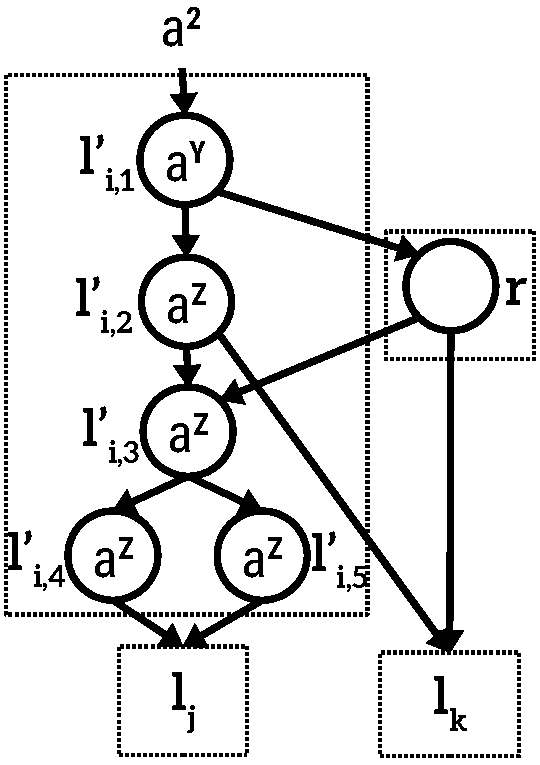
\includegraphics[scale=0.50]{figures/sub-module-2.pdf}
\caption{SUB Module for Simulating Instruction $l'_i:(SUB(r), l_j, l_k)$}
\label{fig-sub}
\end{center}
\end{figure}   

The SUB operation is triggered by sending 2 spikes to neuron $l'_{i,1}$. Neuron $l'_{i,1}$ is the starting neuron of the module. Unlike the ADD
module (for instruction $l_i$) with starting neurons $l_{i,1}$ and $l_{i,2}$, SUB modules only have a single starting neuron. Another difference 
between starting neurons of ADD and SUB module is their initial spikes. i.e. Starting neuron $l'_{i,1}$ of a SUB module will have $y$ initial
spikes while a starting neuron $l_{i,1}$ of an ADD module will have $x$ initial spikes. A common behavior of the starting neurons (for either SUB 
or ADD module) is that they can only use spiking rules by having two spikes. You can only trigger a module operation by sending 2 spikes to all
of its starting neurons.

Let $t$ be the time the 2 spikes are received by starting neuron $l'_{i,1}$. The SUB operation works as follows:

\begin{itemize}
   \item Time: $(t+1)$. Neuron $l'_{i,1}$ will now have $y+2$ spikes and will use \texttt{Rule 4}: $a^{y+2}/a^2 \rightarrow a$ consuming two spikes
                        and sending one spike each to neuron $l'_{i,2}$ and neuron $r$.
   \item Time: $(t+2)$. Neuron $l'_{i,2}$ will now have $z+1$ spikes and will use \texttt{Rule 5}: $a^{z+1}/a \rightarrow a$ consuming one spike and
                        sending one spike each to neuron $l'_{i,3}$ and starting neuron(s) of module $l_k$. If register $r$ is storing number $n$,
                        then neuron $r$ will now have $z+1+3n$ spikes after receiving a spike from neuron $l'_{i,1}$. If $n>0$, neuron $r$ will use 
                        \texttt{Rule 7}: $a^{z+1}(a^3)^+/a^4 \rightarrow \lambda$ consuming 4 spikes and reducing the spike count to $z+3(n-1)$. This
                        decrements the number stored in register $r$ by 1. In this case ($n>0$), SUB operation is successful and only one spike each
                        (from neuron $l'_{i,2}$) will be sent to starting neuron(s) of module $l_k$ so the module will not activate. If $n=0$, neuron
                        $r$ will use \texttt{Rule 5}: $a^{z+1}/a \rightarrow a$ consuming a spike and sending one spike each to starting neuron(s) of
                        module $l_k$. In this case ($n=0$), SUB operation is not successful and starting neuron(s) of module $l_k$ will receive 2 
                        spikes each (1 from neuron $r$ and 1 from neuron $l'_{i,2}$) so the module will activate. Neuron $r$ is also connected to 
                        starting neurons ($l'_{k',1}$) of all other SUB modules that operate on register $r$. These SUB modules' starting neurons
                        $l'_{k',1}$ will only receive one spike changing their spike count from $y$ to $y+1$ which will activate \texttt{Rule 3}:
                        $a^{y+1}/a \rightarrow \lambda$.
   \item Time: $(t+3)$. Neuron $l'_{i,3}$ will either have $z+1$ spikes or $z+2$ spikes. If neuron $l'_{i,3}$ has $z+1$ spikes, the SUB operation is
                        successful and neuron $r$ used \texttt{Rule 7} at time $(t+2)$. In this case, neuron $l'_{i,3}$ will use \texttt{Rule 5}: 
                        $a^{z+1}/a  \rightarrow a$ consuming one spike and sending one spike to neurons $l'_{i,4}, l'_{i,5}$. If neuron $l'_{i,3}$
                        has $z+2$ spikes, then the SUB operation is not successful and neuron $r$ used \texttt{Rule 5} at time $(t+2)$. In this case,
                        neuron $l'_{i,3}$ will use \texttt{Rule 6}: $a^{z+2}/a^2 \rightarrow \lambda$ consuming 2 spikes.
   \item Time: $(t+4)$. If the SUB operation is successful, neurons $l'_{i,4}$ and $l'_{i,5}$ will now have $z+1$ spikes each. They will both use 
                        \texttt{Rule 5}: $a^{z+1}/a  \rightarrow a$ consuming one spike and sending a spike each to starting neuron(s) of module 
                        $l_j$. Each starting neuron(s) of module $l_j$ would receive 2 spikes thus activating the module.
\end{itemize}

% ================================================================================================================================================== %

Based on the SUB operation described above, activating the SUB module for instruction $l'_i:(SUB(r),l_j,l_k)$ (by sending 2 spikes to its starting 
neurons  $l'_{i,1}$) will result in sending $1$ spike to neuron $r$ which will lead to either (1) a successful SUB operation where the value in 
register $r$ was decremented by 1 then module $l_j$ is activated or (2) register $r$ already stores 0 and module $l_k$ is activated.


The OUT operation will halt the execution of instructions and will produce the spike train that represents the output computed by the register 
machine $M$. The OUT operation involves the HALT module, OUT module and neuron $r$ for the output register of the system. HALT module contains 
neurons $l_{h,1}$ and $l_{h,2}$ while the OUT module contains neurons $out'$ and $out$. See Figure \ref{fig-halt} for the other details.

% ================================================================================================================================================== %
   
\begin{figure}
\begin{center}
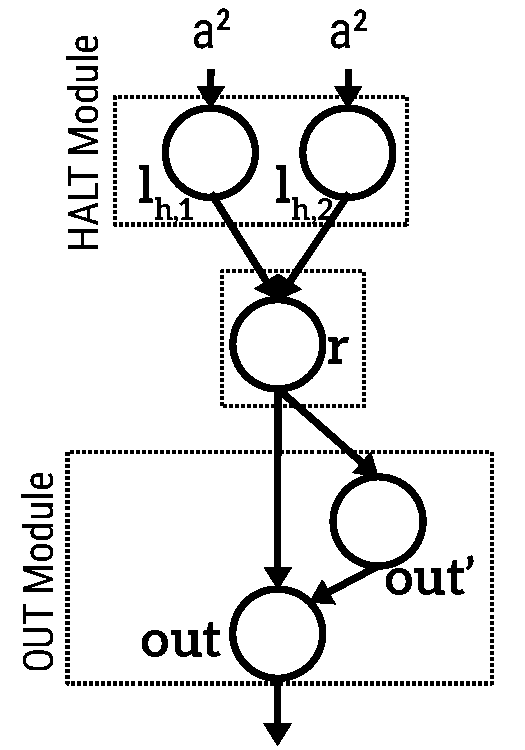
\includegraphics[scale=0.50]{figures/fin-module-2.pdf}
\caption{HALT Module for Simulating Halt Instruction $l_h$ and OUTPUT Module of the System}
\label{fig-halt}
\end{center}
\end{figure}   

The OUT operation is triggered by sending two spikes each to HALT module's starting (and only) neurons $l_{h,1}$ and $l_{h,2}$. Let $t$ be the time
the starting neurons of HALT module received the spikes. The OUT operations work as follows:
\begin{itemize}
   \item Time: $(t+1)$. Neurons $l_{h,1}$ and $l_{h,2}$ will have $y+2$ spike each and both will use \texttt{Rule 4}: $a^{y+2}/a^2 \rightarrow a$
                        consuming two spikes each and sending one spike each to neuron $r$.
   \item Time: $(t+2)$. If at time $t+1$, register $r$ was storing number $n$, represented as $z+3n$ spikes at neuron $r$, then neuron $r$ will now
         have $z+2+3n$ spikes. Neuron $r$ will activate \texttt{Rule 8}: $a^{z+2}(a^3)^+/a^3 \rightarrow a$ consuming 3 spikes and sending one spike 
         each to neurons $out'$ and $out$ of the OUT module. The spikes in neuron $r$ is reduced from $(z+2+3n)$ to $(z+2+3(n-1))$. 
   \item Neuron $r$ will repeatedly use \texttt{Rule 8}: $a^{z+2}(a^3)^+/a^3 \rightarrow a$ consuming $3$ spikes and sending one spike each to 
         neurons $out'$ and $out$. Starting from $(z+2+3n)$ spikes, the spike count will be reduced to $(z+2+3(n-1))$, then to $(z+2+3(n-2))$, then 
         to $(z+2+3(n-3))$ and so on.
   \item After using \texttt{Rule 8} for $n$ times, the spike count in neuron $r$ will be reduced to $z+2$. Neuron $r$ will activate 
         \texttt{Rule 6}: $a^{z+2}/a^2 \rightarrow \lambda$ consuming 2 spikes reducing the spike count to $z$.
   \item In the OUT module, at time (t+3) neuron $out$ will have one spike from neuron $r$ and it will activate \texttt{Rule 5}: $a^{z+1}/a 
         \rightarrow a$ consuming one spike and sending one spike to the environment. At time $(t+4)$ to time $(t+4+n-2)$, neuron $out$ will have 2 
         spikes, one from neuron $r$ and another from neuron $out'$. Neuron $out$ will then activate \texttt{Rule 6}: $a^{z+2}/a^2 \rightarrow 
         \lambda$ forgetting two spikes. At time $(t+4+n-1)$, neuron $out$ will only have one spike received from neuron $out'$. Neuron $out$ will 
         then activate \texttt{Rule 5}: $a^{z+1}/a \rightarrow a$ consuming a spike and sending a spike to the environment for the last time.
         Observing neuron $out$, it sent its first spike to the environment at time $t+3$ and the second (and last) spike at time $(t+n+4-1)$. The
         time difference between these two spikes is $(t+4+n-1)-(t+3)=n$ which is the number generated by the SNPSP system $\Pi$.
\end{itemize}


% ================================================================================================================================================== %

From the behavior of the ADD, SUB, HALT, and OUT modules, we can see that together they can build an SNPSP system $\Pi$ that can simulate the
behavior of a register machine $M$. $\square$ 

% ================================================================================================================================================== %

\subsection{Universality of Homogeneous SNPSP Systems in Accepting Mode}\label{sec-accept}.
\begin{theorem} \label{theorem-2}
$NRE = N_{acc}HSNPSP$ 
\end{theorem}
  
\proof Using the same technique in the proof of Theorem \ref{theorem-1}, it would be sufficient to show that $NRE \subseteq N_{acc}HSNPSP$. For the
converse inclusion $N_{acc}HSNPSP$ $\subseteq NRE$, we can invoked the Church-Turing thesis (similar to the argument in the proof of Theorem 
\ref{theorem-1}. We will construct a homogeneous SNPSP system $\Pi$ that simulates a register machine $M=(m, H, l_0, l_h, I)$ working in accepting mode.

We can use the same modules introduced in Section \ref{sec-gen-mode}. We only need to construct an input module that will take the spike train
$10^{n-1}1$ (time difference between the spikes is $n$) and store the number ($n$) in the designated input register $r$. This input module will
also start the computation of the register machine.

Figure \ref{fig-input} shows the details of the INPUT module.

\begin{figure}
\begin{center}
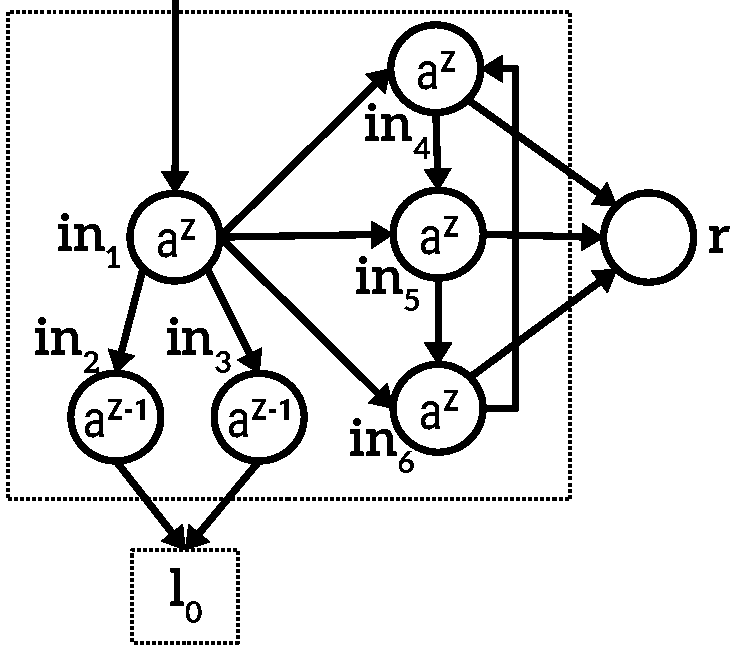
\includegraphics[scale=0.50]{figures/input-module-2.pdf}
\caption{INPUT Module}
\label{fig-input}
\end{center}
\end{figure}   

The INPUT module works as follows:

\begin{enumerate}
   \item Neuron $in_1$ receives the spike train $10^{n-1}1$ from the environment. Let assume the first spike is already at neuron $in_1$ time $0$
         then second spike will be in the neuron at time $n$. At time $0$, neuron $in_1$ will activate \texttt{Rule 5}: $a^{z+1}/a \rightarrow a$  
          sending one spike each to neurons $in_2, in_3, in_4, in_5,$ $ in_6$.
   \item At time $1$, neurons $in_4, in_5, in_6$ have $z+1$ spikes (the additional spike coming from neuron $in_1$). They will all use 
         \texttt{Rule 5} $a^{z+1}/a \rightarrow a$. Neuron $in_4$ will send a spike to neuron $in_5$, neuron $in_5$ will send a spike to neuron
         $in_6$ and neuron $in_6$ will send a spike to neuron $in_4$. These 3 neurons will also send a spike each to neuron $r$. This will increment
         the number stored in register $r$ by 1. Also at time $1$, from the initial $z-1$ spikes neurons $in_2$ and $in_3$ will now have $z$ spikes.
   \item Neurons $in_4, in_5, in_6$ will continue `exchanging' spikes (using \texttt{Rule 5}) and providing spikes to neuron $r$ 3 spikes at a time.
         Neurons $in_4, in_5, in_6$ will do these up to time $n$. This will have the result of incrementing the content of register $r$ (initially 0)
         by $n$.
   \item At time $n$, the second spike is at neuron $in_1$. Neuron $in_1$ uses \texttt{Rule 5}: $a^{z+1}/a \rightarrow a$ consuming a spike and 
         sending a spike to neurons $in_2,in_3, in_4,$ $in_5, in_6$.
   \item At time $n+1$, neurons $in_2, in_3$ will now have $z+1$ spikes and will activate \texttt{Rule 5}: $a^{z+1}/a \rightarrow a$ consuming a spike 
         each and sending one spike each to starting neuron(s) of module $l_{0}$. This will start the computation of the register machine. Also 
         at time $n+1$, neurons $in_4, in_5, in_6$ will have $z+2$ spikes each and all of them will activate \texttt{Rule 6}: $a^{z+2}/a^2 \rightarrow 
         \lambda$ which consumes 2 spikes per neuron.
\end{enumerate}

From the described behavior of the INPUT module, after feeding the spike train $10^{n-1}1$ to the INPUT module via neuron $in_1$, the module was able
to increment the number in register $r$ by $n$. After receiving the two spikes from the environment, the INPUT module was able to start the 
computation by sending two spikes to the starting neuron(s) of module $l_0$ (of the initial instruction $l_0$). The construction of the INPUT module
completes the proof of Theorem \ref{theorem-2}. $\square$
   
% ================================================================================================================================================== %



\section{Discussion and Conclusions} \label{sec-disc}

The values $x,y,z$ that are specified in the rules and as initial spike counts can have any values as long as the values do not make the languages
defined by regular expressions intersect. i.e. For \texttt{Rule 4:} $a^{y+2}/a^2 \rightarrow a$ and \texttt{Rule 5:} $a^{z+1}/a \rightarrow a$, if 
$y=1, z=2$, then the rules will be \texttt{Rule 4:} $a^{1+2}/a^2 \rightarrow a$ and \texttt{Rule 5:} $a^{2+1}/a \rightarrow a$ and the languages
defined by their regular expressions intersect. This is not allowed. Also, the $x,y,z$ values should allow some spike count `gaps'. i.e. For neurons
with initial spike $z$, spike count $z$ is a gap where no rules should be applicable. i.e. If $z=10, y=8$, then \texttt{Rule 4}: $a^{y+2}/a^2 
\rightarrow \lambda$ will be \texttt{Rule 4}: $a^{8+2}/a^2 \rightarrow \lambda$ which will then be used by neurons with initial spike count $z$. This
is not allowed. An example of valid values for $x,y,z$ is $x=0, y=3, z=6$.

The constructed systems use a rule set with 8 rules. In terms of neuron count, an ADD module has 6 neurons (7 if you include neuron $r'$ which is more
associated with register $r$), a SUB module has 5 neurons, an HALT module and an OUT modules have 4 neurons combined, and the INPUT module has 6 
neurons. We can compare this with a closely related homogeneous SNP system in \cite{HSNP}, the system in \cite{HSNP} has a rule set of with 7 rules. In
terms of neuron count, its ADD module has 9 neurons, a SUB module has 5 neurons, the FIN module (similar to HALT+OUT) has 8 neurons, and an INPUT 
module has 14 neurons. The homogeneous SNPSP (HSNPSP) system has 1 more rule than the homogeneous SNP (HSNP) system but has fewer neurons. HSNPSP system
uses generalized forgetting rules and spiking rules while HSNP system uses standard forgetting rules and spiking rules with delay (at most 1 step 
delay).

One challenge in creating homogeneous SNPSP system lies in the nature of the plasticity rule. The component $N$ of the plasticity rule $E/a^c 
\rightarrow \alpha k(i,N)$ specifies a set of target neurons. Essentially, some information about the (possible) local topology of the system is 
encoded in the $N$ component of the rule. The issue is when combining different rule sets you may observe that many rules from different rule sets 
have similar behavior but the rules are technically different because they have a different set $N$ of target neurons.

For example, consider a different ADD module design for some instruction $l_i: (ADD(r), l_j, l_k$). In this new ADD module design, we have a neuron 
$p_i$ with a single plasticity rule $a \rightarrow \pm1(p_i, \{l_{j,1}, l_{k,1}\})$. The function of neuron $p_i$ is to non-deterministically select 
which of possible next instructions to execute by non-deterministically creating a synapse (then deleting it) to either neuron $l_{j,1}$ or 
neuron $l_{k,1}$ and sending a spike to the selected neuron. For two instructions $l_a: (ADD(r), l_b,l_c)$ and $l_d:(ADD(r'), l_d, l_e)$, ADD module
for $l_a$ will have neuron $p_a$ with the rule $a \rightarrow \pm1(p_a,\{l_{b,1}, l_{c,1}\})$ while ADD module for $l_d$ will have neuron $p_b$ with
the rule $a \rightarrow \pm1(p_d,\{l_{e,1}, l_{f,1}\})$. This means that for each instruction $l_i$ with different sets of possible next instructions 
(i.e. different $l_j, l_k$), the module for $l_i$, specifically neuron $p_i$, will have a unique rule set containing only  the rule $a \rightarrow \pm1(p_i,
\{l_{j,1}, l_{k,1}\})$. These rules, though having the same purpose of selecting the next ins:w
truction to execute, can not be represented by a single
rule in the homogeneous rule set because they have local-only relevant information. i.e. The set of target neurons representing the possible next
instructions is relevant only to the module of some specific instruction.

The universal SNPSP systems constructed in Section \ref{homogeneous-snpsp} only use the plasticity rule $E/a^c \rightarrow -1(i,\{x\})$ to simulate
the function of an SNP system's forgetting rule. Written as $E/a^c \rightarrow \lambda$, this SNPSP system's forgetting rule is more general than
an SNP system's forgetting for reasons described in Section \ref{sec-forget}. This implies that it is possible to construct a universal SNPSP system
with plasticity rules that uses only $\alpha = -$ or more generally one type of action (plasticity rules with $\alpha = +$ can also simulate 
forgetting rules). It also implies that SNPSP system's spiking rules and  generalized forgetting rules are enough for universality.

% ================================================================================================================================================== %



\section*{Acknowledgements}
R.T.A. de la Cruz and I.C.H. Macababayao  are grateful for the Philippine's Department of Science and Technology - Science Education Institute (DOST-SEI)'s support 
through the Engineering Reasearch and Development for Technology (ERDT)'s graduate scholarship program.
F.G.C. Cabarle thanks the support from the DOST-ERDT project; the Dean Ruben A. Garcia PCA AY2018--2019, and an RLC AY2018--2019 grant of the OVCRD, both from UP Diliman.
H. Adorna would like to thank supports from DOST-ERDT project since 2009 until present; the Semirara Mining Corp. Professorial Chair Award since 2015 until present. The RLC  grant from UPD - OVCRD 2019-2020.
The work was supported by the Basic Research Program of Science and Technology of Shenzhen (JCYJ20180306172637807).


% ================================================================================================================================================== %

\bibliographystyle{splncs03}
\bibliography{cmc20-paper9}

\end{document}
